\documentclass{article}[12pt]

%--------------Packages------------------------------
\usepackage[utf8]{inputenc} %Pour encoder du texte en français
\usepackage[francais]{babel} %Pour encoder du texte en français
\usepackage{graphicx} %pour inclure des images
\usepackage{changepage}
\usepackage{version} % permet d'utiliser l'environnement comment
\graphicspath{{./figures/}} %repertoire images
\usepackage{listings} %si on veut afficher du code, le code doit se trouver dans un dossier "codes" 					  %lui même dans le même répertoire que ce fichier tex
\usepackage{color} %nécessaire pour changer les couleurs du highlighting du code
\usepackage{amsmath,amssymb}%pour des maths au cas où
\usepackage{array,multirow,makecell}%Pour manipuler les tableaux
\usepackage{url} %pour utiliser les liens hypertextes
\usepackage{hyperref} %pour utiliser les liens hypertextes
\usepackage{float}
\newlength{\offsetpage}
\setlength{\offsetpage}{2.0cm}
\usepackage[left=2cm,right=2cm,top=2cm,bottom=2cm]{geometry}
\newenvironment{widepage}{\begin{adjustwidth}{-\offsetpage}{-\offsetpage}%
    \addtolength{\textwidth}{2\offsetpage}}%
{\end{adjustwidth}}

\newcommand{\Java}[2]{
	\begin{itemize}
    	\item[]\lstinputlisting[caption=#2,label=#1]{#1.java}
	\end{itemize}
}
% ---------- Document ------------ %
\begin{document}

\begin{titlepage}

\newcommand{\HRule}{\rule{\linewidth}{0.5mm}} % Defines a new command for the horizontal lines, change thickness here

\center % Center everything on the page
 
%----------------------------------------------------------------------------------------
%	HEADING SECTIONS
%----------------------------------------------------------------------------------------

\textsc{\LARGE Institut Paul Lambin}\\[1.5cm] % Name of your university/college
\textsc{\Large BAC 2 Informatique de gestion}\\[0.5cm] % Major heading such as course name
\textsc{\large Unix}\\[0.5cm] % Minor heading such as course title

%----------------------------------------------------------------------------------------
%	TITLE SECTION
%----------------------------------------------------------------------------------------

\HRule \\[0.4cm]
{ \huge \bfseries Synthèse Unix }\\[0.4cm] % Title of your document
\HRule \\[1.5cm]
 
%----------------------------------------------------------------------------------------
%	AUTHOR SECTION
%----------------------------------------------------------------------------------------

\begin{minipage}{0.4\textwidth}
\begin{flushleft} \large
\emph{Auteurs:}\\
Christopher \textsc{Sacré} \\ % Your name
\end{flushleft}
\end{minipage}
~
\begin{minipage}{0.4\textwidth}
\begin{flushright} \large
\emph{Professeur:} \\
C. \textsc{De Muylder}\\
B. \textsc{Henriet}\\
A. \textsc{Ninane}% Supervisor's Name

\end{flushright}
\end{minipage}\\[4cm]

% If you don't want a supervisor, uncomment the two lines below and remove the section above
%\Large \emph{Author:}\\
%John \textsc{Smith}\\[3cm] % Your name

%----------------------------------------------------------------------------------------
%	DATE SECTION
%----------------------------------------------------------------------------------------

{\large \today}\\[3cm] % Date, change the \today to a set date if you want to be precise

%----------------------------------------------------------------------------------------
%	LOGO SECTION
%----------------------------------------------------------------------------------------

%\includegraphics{Logo}\\[1cm] % Include a department/university logo - this will require the graphicx package
 
%----------------------------------------------------------------------------------------

\vfill % Fill the rest of the page with whitespace

\end{titlepage}

\tableofcontents%table des matières
\newpage
\section{Prise de Notes}
\subsection{Semaine 2}
\subsubsection{Introduction à l'architecture}
\begin{figure}[H]
	\fbox{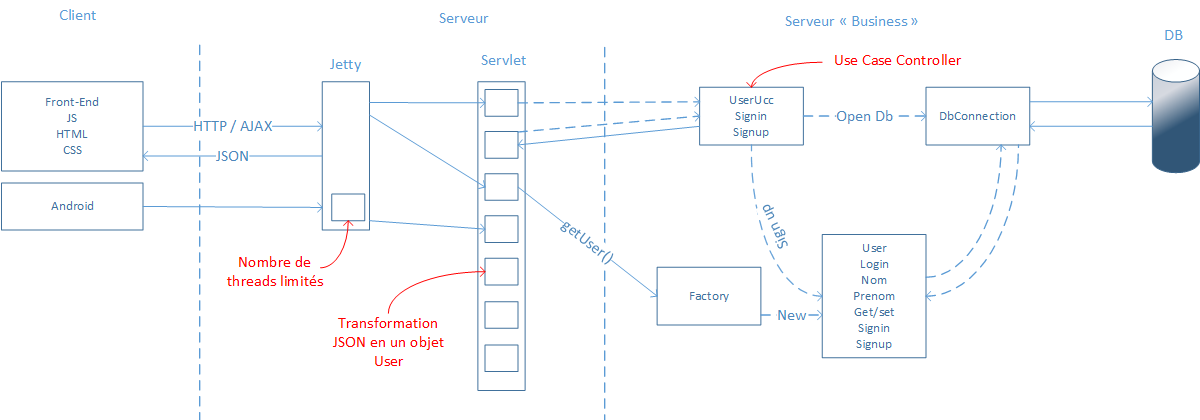
\includegraphics[scale=0.53]{Schema_2.png}}
    \centering
    \caption{Introduction du cours}
\end{figure}
\subsubsection{Informations}
Si vous souhaitez des informations supplémentaires, plusieurs logiciels ont été mentionné durant ce cours : Harmony, Visual Studio Code ainsi que Electron. (Il s'agit d'un cours nous introduisant les concepts de notre application ainsi que les bases de son architecture).
\subsection{Semaine 3}
\subsubsection{Traitement d'un UseCase}
\begin{figure}[H]
	\fbox{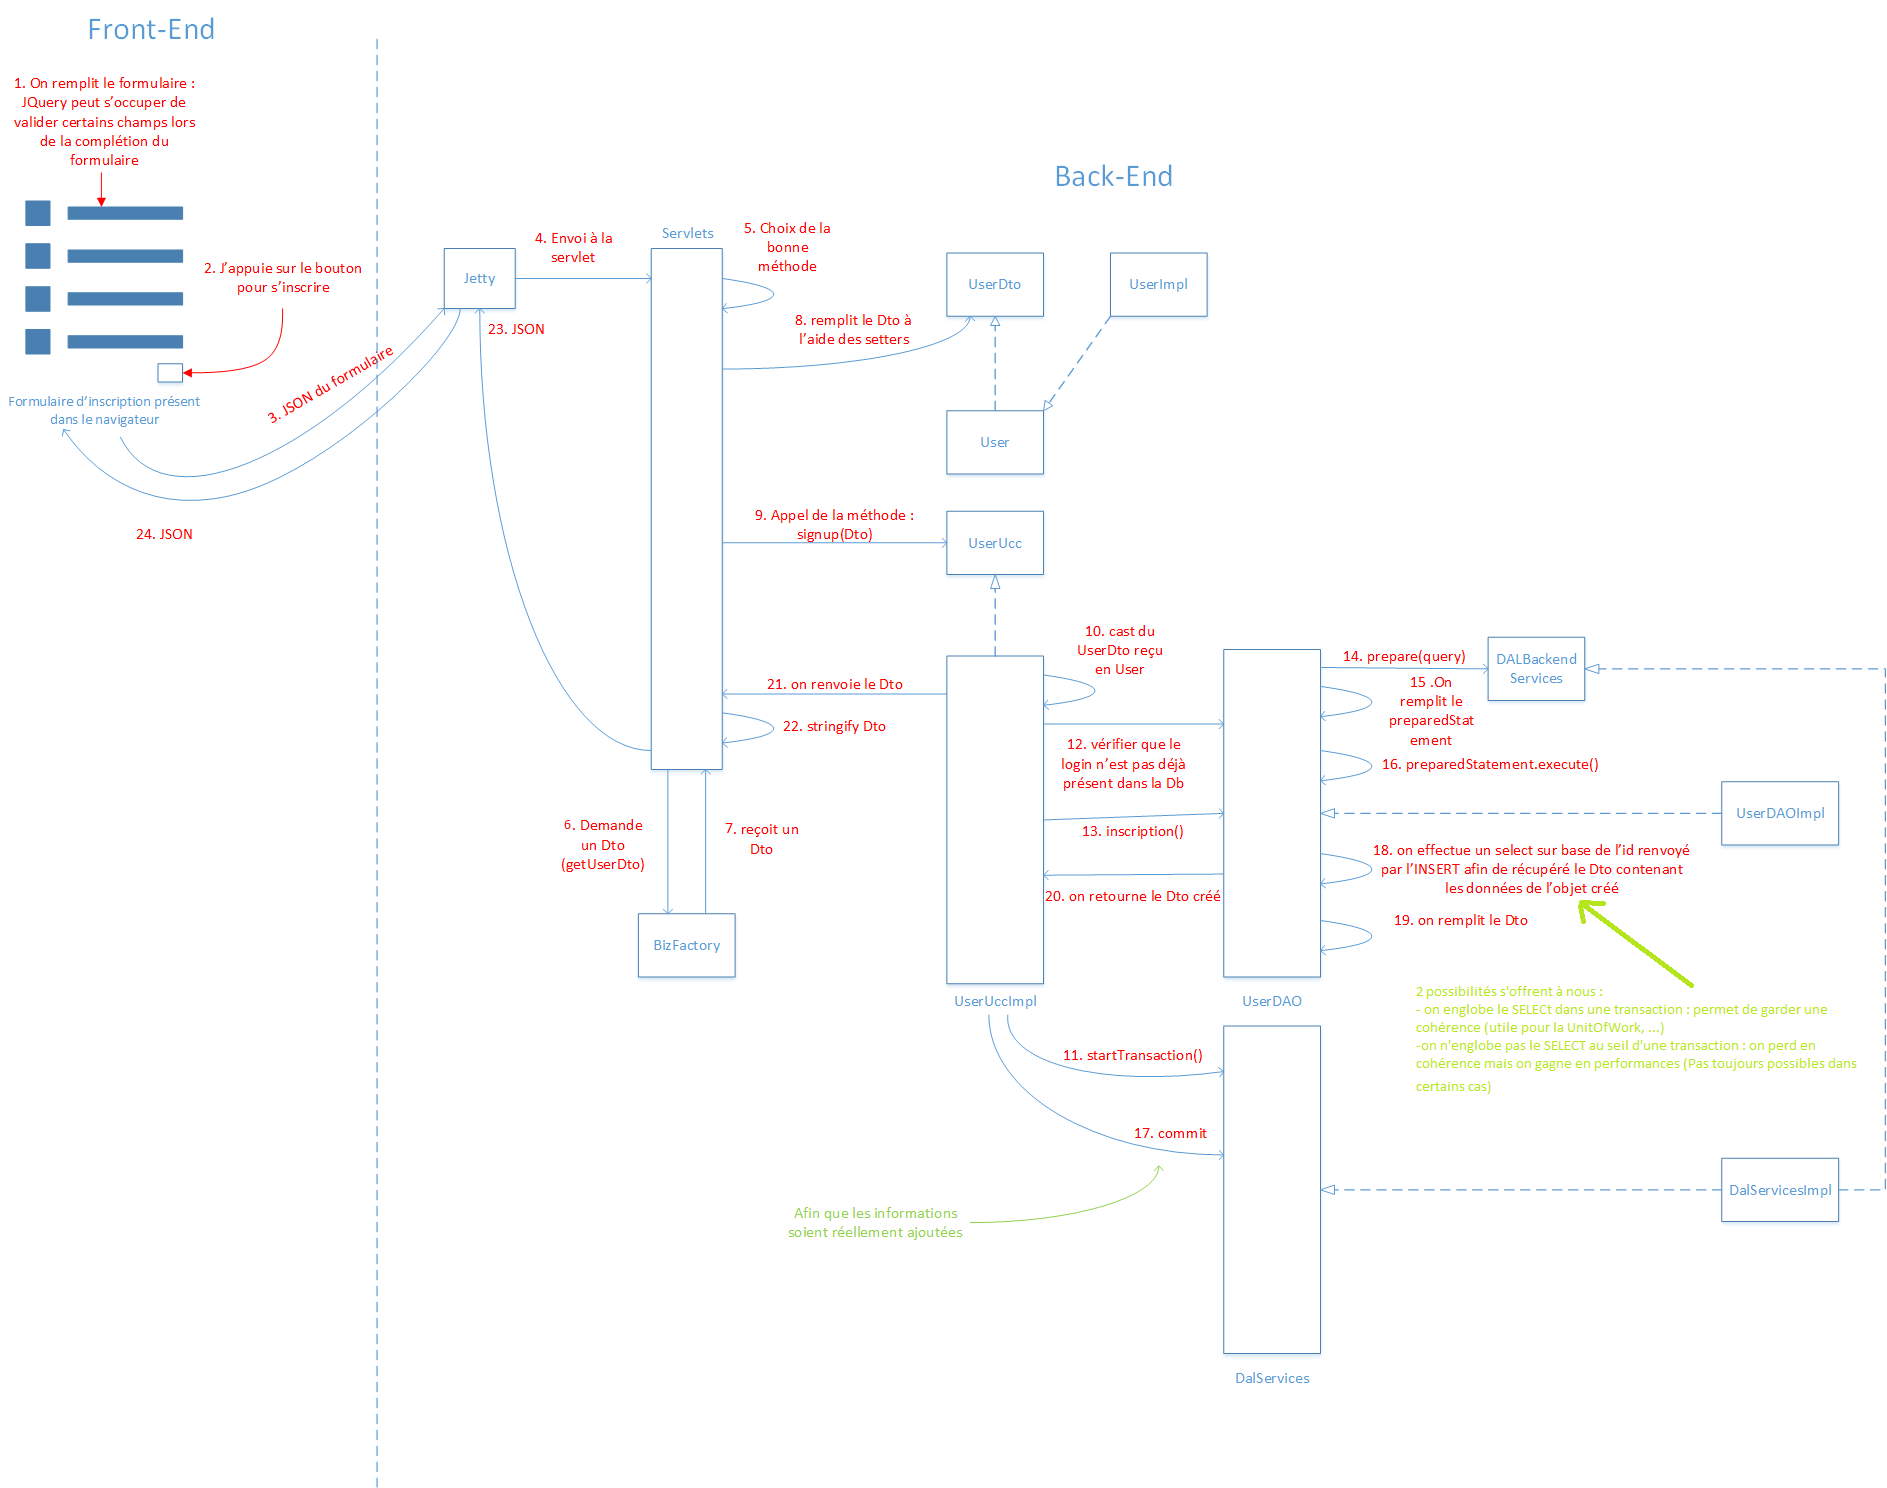
\includegraphics[scale=0.35]{Schema_3.png}}
    \centering
    \caption{Exemple d'utilisation de notre architecture (UC : s'inscrire)}
\end{figure}
\subsection{Semaine 4}
\subsubsection{Architecture Monothread complète}
\begin{figure}[H]
	\fbox{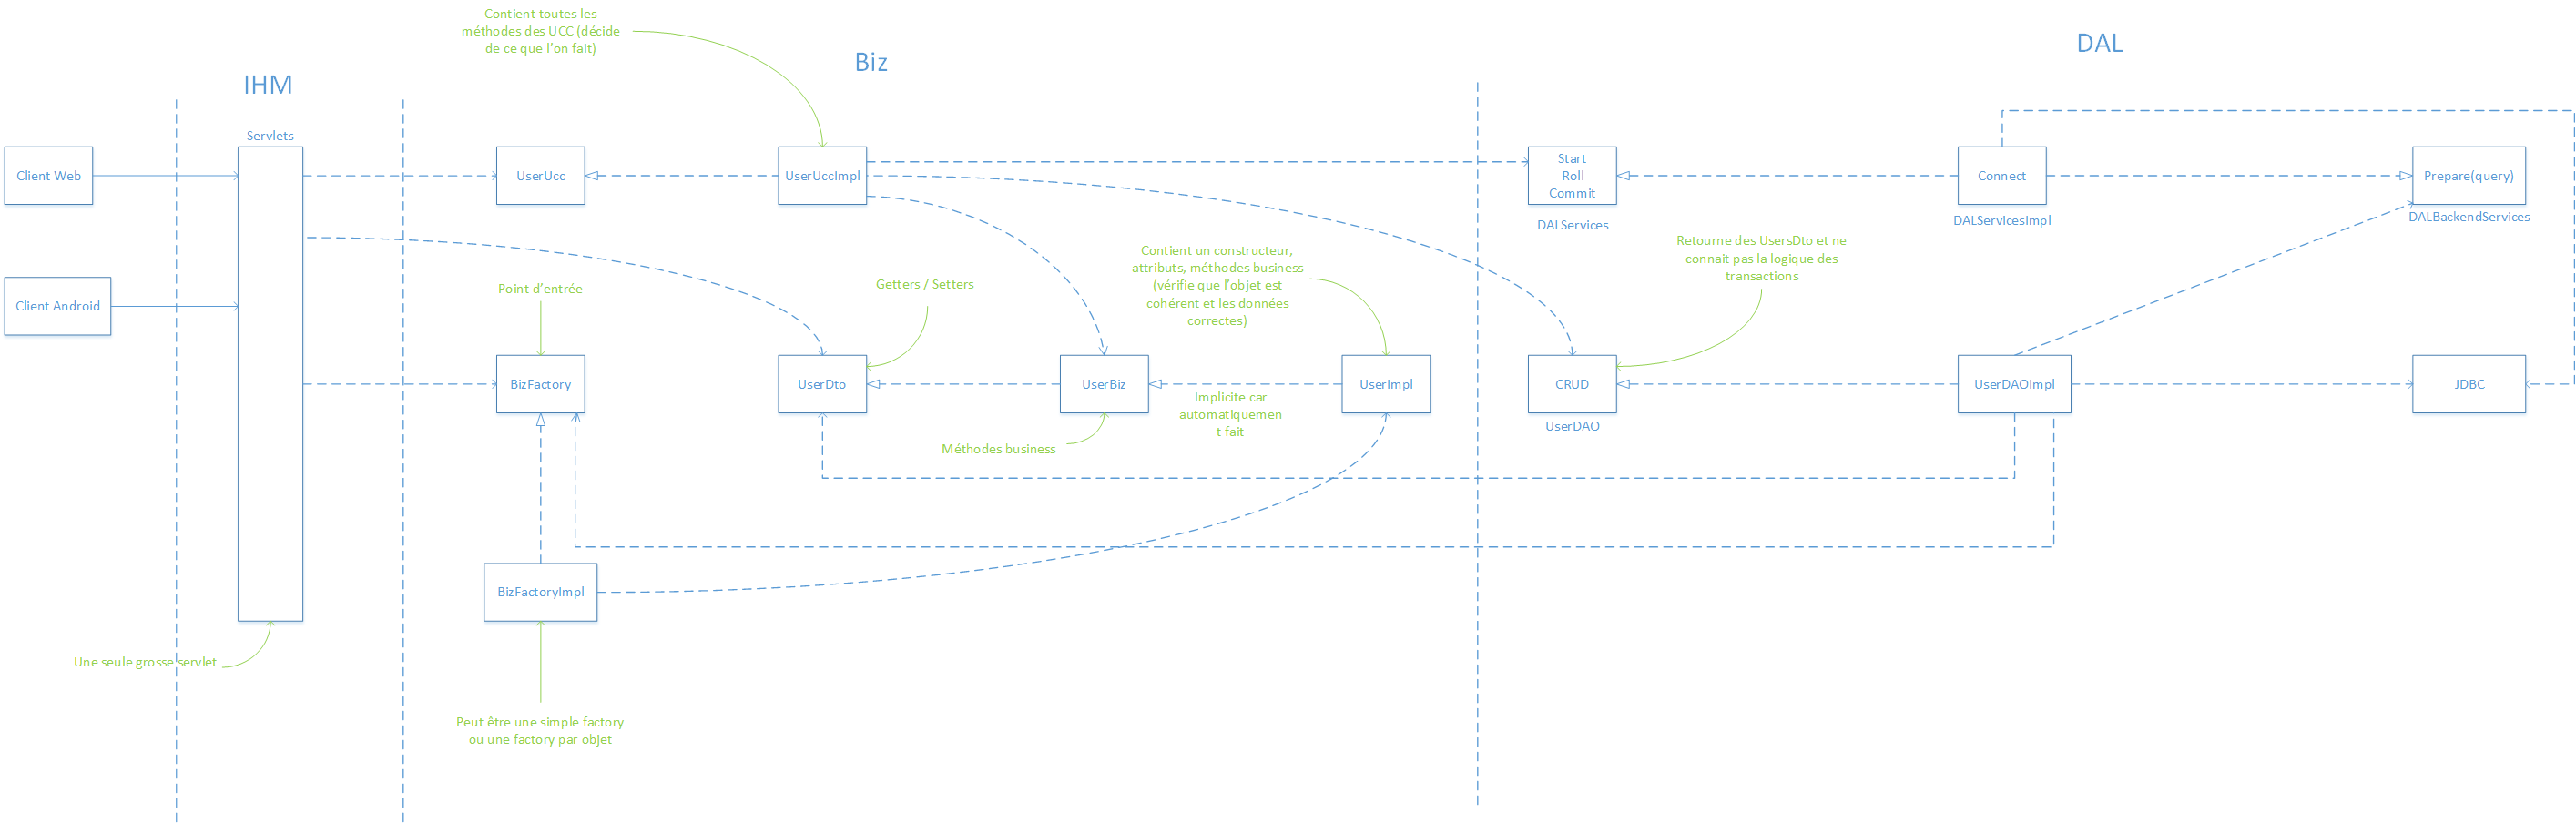
\includegraphics[scale=0.25]{Schema_4.png}}
    \centering
    \caption{Architecture Monothread complète}
\end{figure}
\subsubsection{Informations complémentaires} 
\paragraph{Factoring : } Il faut savoir que l'on mettra de nombreuses classes, ... public mais on tentera d'utiliser uniquement les points d'entrées (surtout au sein de la couche IHM), dans le même style, on utilisera de nombreuses interfaces afin de diminuer le nombre de dépendances concrètes et faciliter le changement entre l'environnement de prod et celui de dev. Par ailleurs, la servlet ne doit pas connaitre les méthodes bussiness (Car dans le cas contraire elle pourrait les modifier). 
\paragraph{Traitement des INSERT : }lorsque l'on insère, on tente de retourner l'entièreté de l'objet crée et non juste l'id, cela permet de vérifier que tout c'est bien passé. 
\paragraph{Traitement des SELECT : } point suivant est plutôt controversé et dépend de votre version des choses il s'agit de l'utilisation de transactions au niveau des select : on peut ne pas utiliser de transaction (perte de cohérence mais gain de performances) ou au contraire utiliser des transactions (perte de performances mais gain de cohérence). 
\paragraph{Sécurité : } Il est important que le back-end soit totalement indépendant du front-end (les données reçues ne sont en aucun cas sure).
\paragraph{Remarque : } un framework nous pose des rails, cela nous permet uniquement de nous orienter , dès lors il faut parfois s'éloigner des rails.
\subsection{Semaine 5}
\paragraph{Main : } Le main permet de démarrer Jetty, c'est lui qui s'occupe de créer les servlets Jetty. Il crée les Factory à l'ai de l'injection de dépendance. Dés que tout cela est créé, il se met en pause (Le main se lance au démarrage de l'application).
\subsection{Semaine 6}
\subsubsection{ConnexionPool}
\begin{figure}[H]
	\fbox{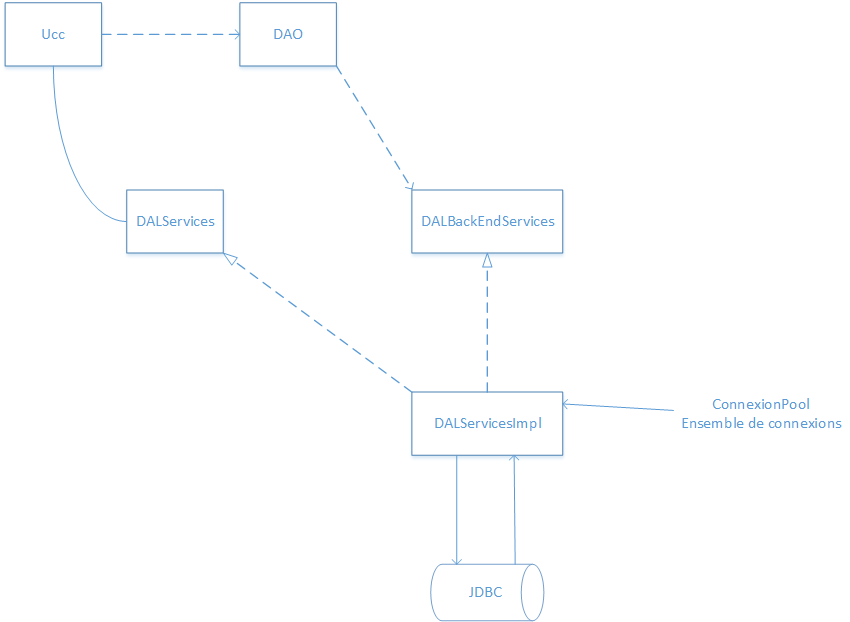
\includegraphics[scale=0.50]{Schema_5.png}}
    \centering
    \caption{Connexion Pool}
\end{figure}
\paragraph{Introduction : } gros problème que l'on a tenté de résoudre est le fait que l'on ne pouvait ouvrir qu'une seule transaction à la fois (Il est totalement interdit d'ouvrir plusieurs transactions sur la même connexion en même temps, En cas de transactions imbriquées, si la première transaction à un soucis le rollback ne se propagera pas, mais s'arrêtera au premier commit). 
\paragraph{Solution : } Jetty à pour cela, un ensemble de Thread (Il n'en a pas un nombre infinis). On va donc remplacer notre précédente unique connexion par un ensemble de connexions (Le nombre de connexions à avoir est de notre ressort, et c'est donc à nous de faie ce choix).
\paragraph{Aide à la solution : } On peut afin de nous aider à implémenter cela utiliser ThreadLocal (On aurait dès lors une connexion par thread, utilisation d 'une Map<Thread, ConnexionDb> (pour cela on peut utiliser la méthode Thread.getId() qui renvoie l'id du threadCourant), ou plus facile encore ou pourrait utiliser la classe ThreadLocal, notre Map deviendrait alors un ThreadLocal<Connexion>, la clé est directement l'id du thread local (il s'agit tout simplement d'une map pour laquelle on a spécifié la syntaxe)). 
\paragraph{Problème : } le problème avec ces deux solutions vient du fait que si il y a une connexion par thread, on va donc multiplier le nombre de connexions (La taille du threadPool est un problème en soit (il faut pouvoir la fixer et cela dépend la plupart du temps fort de la couche Bussiness (Si il n'y a pas assez de Connexions, cela bloquera le thread tant qu'il n'y en aurait pas une de disponible). 
\paragraph{Solution Finale : } Afin de palier à tout cela, on va utiliser DBCP2 (Une librairie Java, DataBaseConnexionPool).
\subsection{Semaine 7}
\subsubsection{Informations}
\paragraph{Affichage des erreurs : } Afin d'afficher des erreurs on peut utiliser System.err.println (La différence avec System.out.println est qu'il pourrait y avoir un décallqge au niveau de l'affichage).
\paragraph{Classe Logger : }\href{https://docs.oracle.com/javase/8/docs/api/java/util/logging/Logger.html}{La classe Logger} permet de définir une priorité au niveau des messages (Il plusieurs niveaux de priorité : SEVERE (valeur la plus élevée), WARNING, INFO, CONFIG, FINE, FINER, FINEST (valeur la moins élevée). L'avantage de cela est que l'on pourrait Logger sur un autre serveur , permettant ainsi d'empêcher la surcharge d'un appareil (Il est intéréssant de Logger : le temps de réponse, le type d'appareil utilisé , le type de route utilisé, ou tout ce qui vous semble intéressant d'être connus). 
\paragraph{Profiler - SQL : } permet de connaitre le temps d'exécution d'une réponse.
\paragraph{Sécurité : } On pourrait rajouter une couche afin d'empêcher les attaques DDOS (Cette couche permettrait de filtrer les requêtes et de les dispatcher à des serveurs plus petit qui traiteraient alors les requêtes).  Un autre point important pour la sécurité est qu'il ne faut jamais faire confiance à l'utilisateur, Il faut par ailleurs faire la distinction entre Admin et Utilisateur et utiliser JWT (cf cours de JavaScript).
\subsection{Semaine 8}
\subsubsection{Optimistic Lock}
\begin{figure}[H]
	\fbox{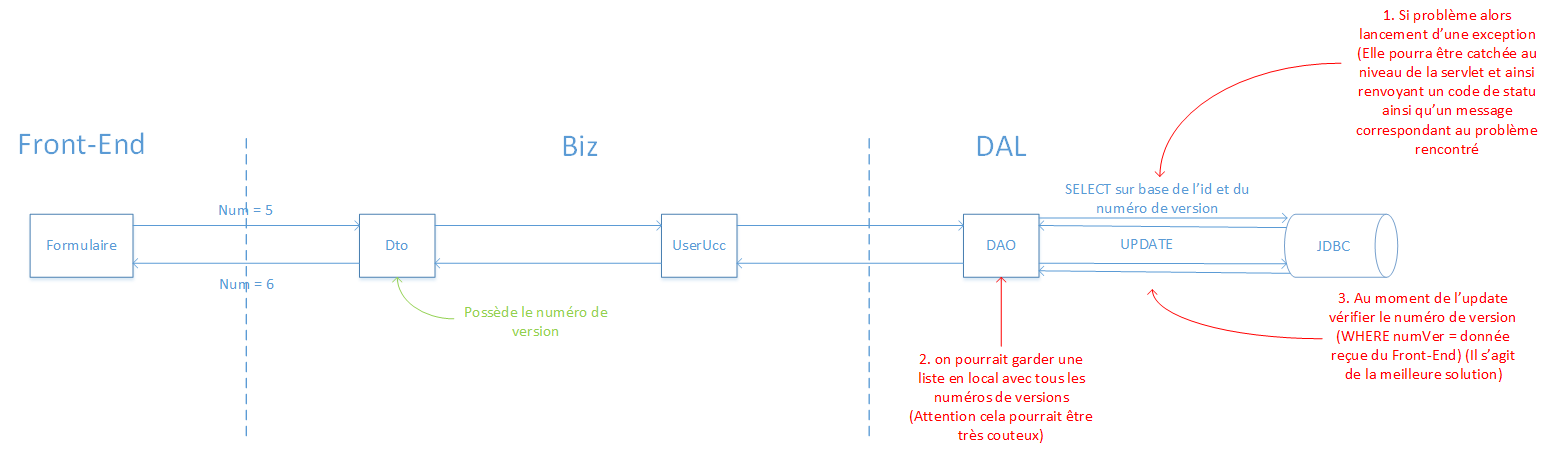
\includegraphics[scale=0.46]{Schema_6.png}}
    \centering
    \caption{Optimistic Lock}
\end{figure}

\paragraph{Introdution : } un gros problème sur ce genre d'applications utilisée par plusieurs personnes est le problème de concurrence (Imaginons que deux personnes affichent la même donnée, le premier la modifie mais le premier qui l'avait également sous les yeux la modifie également, comment savoir quelles données sont correctes ?, comment faire pour que l'application reste cohérente à ce niveau là ?). Il existe deux solutions à cela : l'Optimistic Lock et le Pessimistic Lock (Durant notre cours nous nous intéresseront surtout à l'Optimistic Lock). 
\paragraph{Optimistic Lock : } On va utiliser un numéro de version que l'on va incrémenter à chaque modification (lorsqu'un utilisateur veut modifier une ressource, on récupérera l'id de l'objet ainsi que son numéro de version depuis le front-end et on le comparera avec ceux présent dans la base de données). On a décidé de ne pas travailler avec des timestamps car ils sont peu pratique à utiliser et qu'il peut y avoir un problème de décalage. 
\paragraph{Amélioration possible : Refresh Intermittent}, Une amélioration possible de notre système serait de prévenir le Front-End depuis le Back-End dès qu'une modification a lieu. Le problème vient du fait que normalement seul le client peut parler au serveur (C'est lui qui lance le processus de communication). Pour palier à cela il existe tout de même deux solutions : La solution Web-Socket (on ouvre un tuyau bi-directionnel entre les deux) ou la solution de Calling (on va faire des requêtes successives après un intervalle restreint afin de savoir si il y a eu une modification).
\paragraph{Amélioration possible : Exception }, Une autre amélioration possible serait le lancement d'une exception si les numéros de versions ne correspondent pas, cette dernière serait récupérée au niveau de notre servlet qui pourrait envoyer une erreur correspondant au problème rencontré (ayant pour code d'erreur : 409).
\paragraph{Particularités DELETE : } lors d'une suppression, on ne réalisera jamais de Hard Delete (DELETE en tant que tel sur la base de donnée, car cela pourrait avoir de grosses répercussions imaginons que l'objet supprimé soit référencé dans d'autres objets de la base de données, de plus des normes légales nous oblige à conserver nos données et on pourrait en avoir besoin pour faire des statistiques, ...) mais bien un soft Delete (On mettra juste un flag permettant de savoir si l'objet est supprimé à TRUE).
\paragraph{UnCaughtExceptionHandler : },  \href{https://docs.oracle.com/javase/7/docs/api/java/lang/Thread.UncaughtExceptionHandler.html}{La classe UnCaughtExceptionHandler}  est une classe que l'on peut instancier et assigner à un thread. Cette classe possède une fonction : uncaughtException qui permet si un thread a été stoppé par une exception qui n'a pas été attrapée, de fermer le serveur/ le thread qui l'exécute et d'ainsi permettre l'écriture d'un log afin d'enregistrer le problème.
\subsection{Semaine 9}
\subsubsection{Introduction à la UnitOfWork}
\paragraph{Problème rencontré : } le problème de cette semaine concerne surtout le fait que chaque useCase de notre application nécessitait l'ouverture et la fermeture d'une transaction (dû au commit à chaque fin de UseCase). Cela cause de gros soucis de performances mais pire que cela i lfaut faire attention aux Usecases imbriqués (Il est totalement interdit de faire des startTransaction / commit imbriqués).
\paragraph{Solution : } afin de palier à cela, on va utiliser un intermédiaire qui s'occupera de la logique de transactions (Il s'agira d'une classe à part qui s'occupera de la logique start-commit business). Cette classe s'occupera également de faire les appels aux DAOs, elle stockera les objets en vue d'UPDATE, INSERT et DELETE futur, au moment du commit à proprement parlé (lors de l'appel de la méthode commit de l'intermédiaire), l'intermédiaire va ouvrir la transaction, effectuer les opérations Db et commit. Attention, la UnitOfWork n'est pas nécéssaire pour le Multithreading, il s'agit surtout d'une amélioration pour les performances.
\paragraph{Stockage données : } Etant donné que la classe intermédiaire garde en mémoire tout ce qu'elle doit faire on devra utiliser trois maps (une map pour INSERT, une map pour DELETE, une map pour UPDATE). 
\paragraph{Améliorations au niveau des performances :} Afin d'améliorer les performances on peut lors d'un INSERT et de plusieurs UPDATE sur un même objet, faire directement l'INSERT avec les bonnes données (Il faut faire attention au niveau de la cohérence), Pareil pour de multiples UPDATE, et dans le cas d'un INSERT ou d'un UPDATE suivis d'un DELETE, directement effectué le DELETE. 
\paragraph{Solution Multithreading : } Afin de permettre une solution multithreading on va devoir utiliser un ThreadLocal qui aura comme valeur la liste des trois Maps (Afin de permettre cela on va créer une classe interne (UnitOfWorkBag qui aura comme attributs les trois maps). 
\paragraph{Solution start-commit imbriqués : } On va utiliser une sémaphore (s'incrémentera de un à chaque start transaction de la classe intermédiaire, se diminuera de un à chaque rollBack, commit de la classe). Si la sémaphore est égale à 0 alors on lancera la procédure de commit autrement on effectuera aucun traitement. 
\subsection{Semaine 10}
\subsubsection{Impact de la UnitOfWork}
\begin{figure}[H]
	\fbox{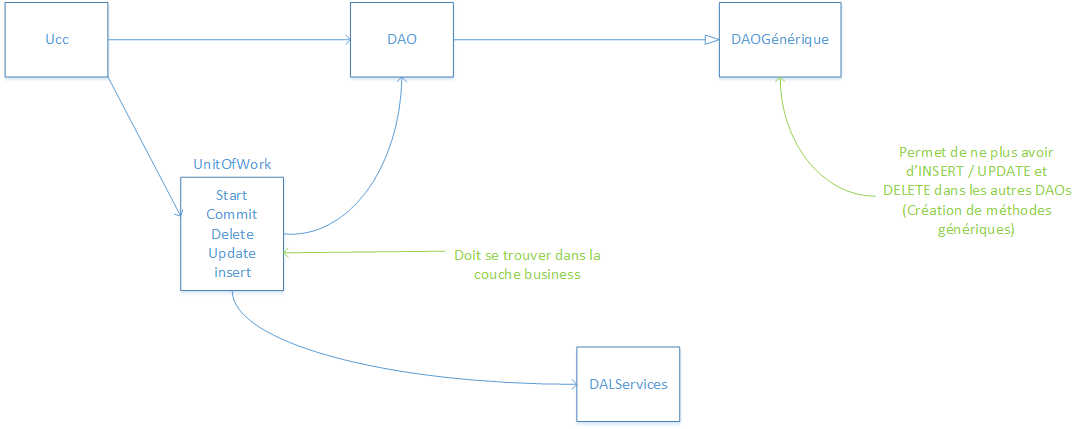
\includegraphics[scale=0.55]{Schema_7.png}}
    \centering
    \caption{Impact de la UnitOfWork}
\end{figure}
\subsubsection{Améliorations de la UnitOfWork}
\paragraph{Améliorations de la UnitOfWork}
\begin{itemize}
	\item \emph{DAO générique :} on va créer un DAO générique qui s'occupera lui même de choisir la table de notre base de données à impacter en fonction de l'objet reçu. (Cette amélioration peut être remplacée par une interface DAO ayant trois méthodes : insert, update et delete ainsi tous nos DAO implémenteront cette interface et il nous suffira de choisir le DAO correspondant sur base de l'objet (afin de permettre cela (nous ne savon pas à l'avance le type d'objet reçu on utilisera l’introspection ainsi qu'un fichier properties (on gardera dans le fichier properties les DAOs responsable de chacun des objets (Afin de savoir de quel objet il s'agit on pourra utiliser la méthode objet.getClass()))).
    \item \emph{Factory DAO : } Elle permettra de conserver la logique de recherche du DAO correspondant.
    \item \emph{ORM : } \href{http://hibernate.org/orm/documentation/5.2/}{ORM} permet de mapper directement les objets java avec les objets en Db, pour cela on précisera sur chaque champs la colonne lui étant reliée (@Column) quant aux champs n'étant pas en rapport avec la db on le précisera à l'aide de l'annotation : @Transient.
    \item \emph{JPA : } \href{https://openclassrooms.com/courses/creez-votre-application-web-avec-java-ee/la-persistance-des-donnees-avec-jpa}{JPA} permet d'être indépendant des bases de données.
    \item \emph{Views} \href{https://docs.microsoft.com/en-us/aspnet/core/mvc/views/dependency-injection}{Views} permet de faciliter l'injection de dépendances.
\end{itemize}
\paragraph{Différents type d'ids : }
\begin{itemize}
	\item \emph{CID : } il s'agit de l'identifiant conceptuel (Conceptual ID). Il s'agit d'un identifiant proche du métier, il est unique au sein d'un type d'objets (PK de l'objet en Db). LE problème avec ce type d'id est que l'on peut avoir des objets de type différents ayant le même cid.
    \item \emph{OID : } il s'agit de l'identifiant de l'objet (Object ID), ce dernier n'est pas utilisé par le client et est unique pour tous les types d'objets, aucun objet n'aura le même oid qu'un autre qu'ils soient de même type ou non à moins d'être égaux.
    \item  \emph{MID : } il s'agit de l'identifiant en mémoire (Memory ID). On ne peut donc en aucun cas se baser dessus.
    \item \emph{UUID : } \href{https://docs.oracle.com/javase/7/docs/api/java/util/UUID.html}{UUID } est une classe java permettant de créer des ids de manière pseudo aléatoire (En utilisant le timestamp courant ainsi que les infos du pc (le nombre de cœurs, la fréquence CPU utilisée actuellement, ....). 
\end{itemize}
\paragraph{Guice} \href{https://github.com/google/guice}{Guice} est une libraire qui permet de faciliter le processus d'injection de dépendances (Pour plus d'informations à ce sujet c'est par \href{https://github.com/google/guice}{ici}.
\subsection{Semaine 11}
\subsubsection{Les Sessions}
\begin{figure}[H]
	\fbox{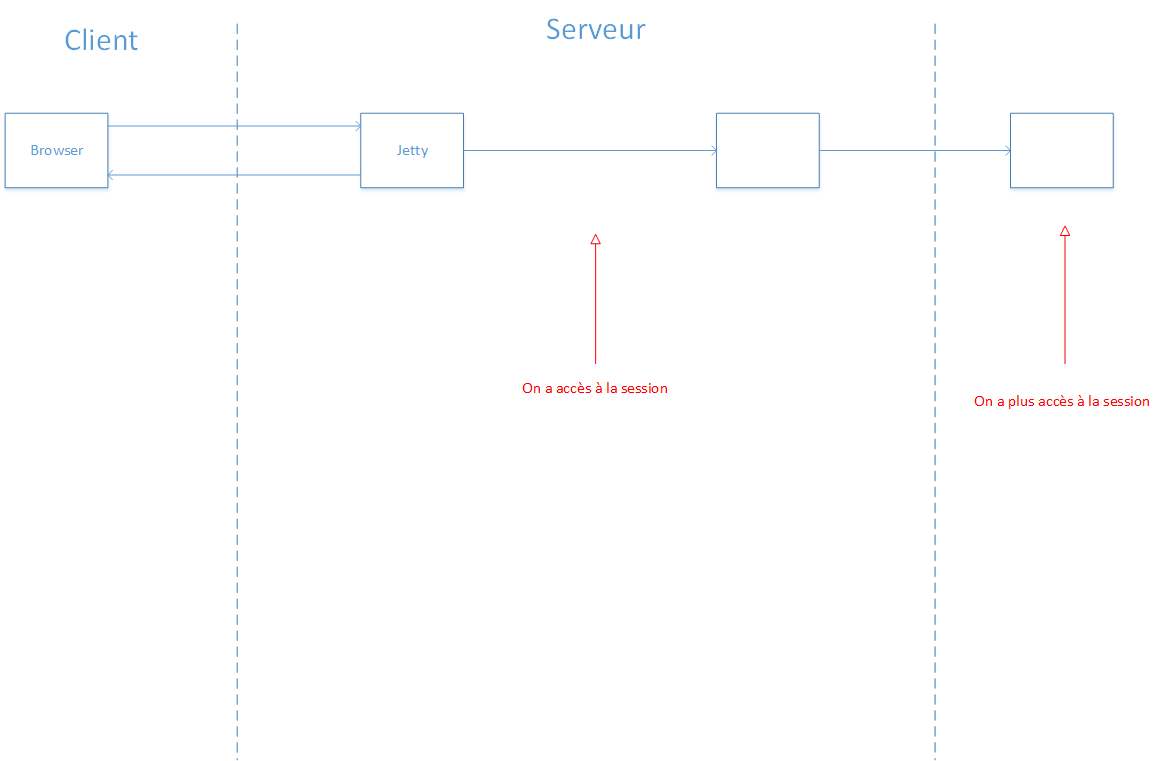
\includegraphics[scale=0.55]{Schema_8.png}}
    \centering
    \caption{Problème avec les sessions}
\end{figure}
\paragraph{Introduction : } les sessions sont plutôt uniformes et communes à plusieurs langages. Elle permettent de garder les infos de la personne qui a effectué la requête (Le token JWT permet identifier l'utilisateur mais également de garder les informations pouvant être utile à chaque requête).
\paragraph{Problème rencontré : } Comment va t'on faire pour avoir accès à cette session au niveau de la couche Business ? On ne peut pas la passer en paramètre (ce serait bien trop fastidieux), ni la mettre dans un fichier properties (cela ne peut se faire quant on à plusieurs utilisateurs).
\paragraph{Solution : Thread} une solution au problème serait de stocker la session dans le thread. Afin d'avoir accès à cette session partout on va créer une classe SessionManager qui aura un attribut de type ThreadLocal (cet attribut pourrait même être statique, mais la dépendance concrète à peu d'importance). 
\paragraph{Classe Config : } on pourrait dès lors créer une classe Config disponible dans toute notre application qui contiendrait des infos devant être accesible un peu partout. 
\end{document}
